\chapter{BIODATA PENULIS}
		\begin{wrapfigure}{l}{0.3\textwidth}
			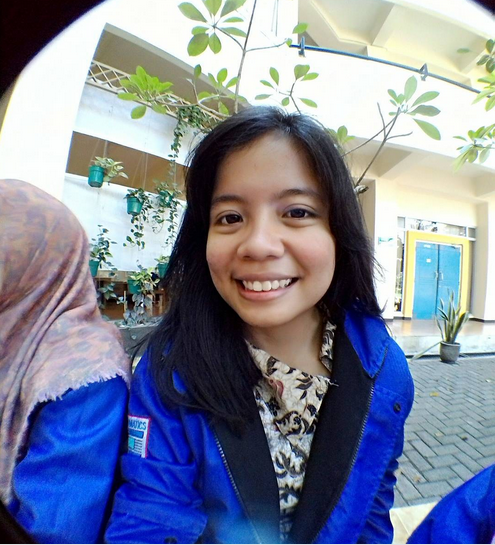
\includegraphics[width=0.3\textwidth]{images/foto-diri.png}
		\end{wrapfigure}
		\textbf{\ \\Ronauli Silva Natalensis S}, kelahiran \& besar di Siantar - Medan, sangat suka belajar. Diberi amanah untuk menjadi \textit{administrator} Laboratorium Pemrograman di tahun 2015, penulis belajar banyak mengenai administrasi \textit{server}, rancang bangun aplikasi terutama di bidang web. Selain itu, beberapa \textit{project} yang diambil penulis mengenai rancang bangun aplikasi yang baik dan buruk yang mengajarkan penulis cara memperbaiki, menangkal dan \& mengoptimasinya.\\
		Selain itu, penulis juga banyak belajar \textit{softskills} saat diamanahi menjadi sekretaris departemen HMTC ITS 2015/2016 dan juga lewat pelatihan-pelatihan beswan Karya Salemba Empat 2014-2016.\\
		\indent Motto penulis yaitu "\textit{Always go for the extra miles}", membawa penulis mengambil topik tugas akhir ini, dimana penulis dapat menerapkan perbaikan, optimasi dan pelajaran yang penulis petik dari \textit{project-project} sebelumnya, dengan bimbingan dosen-dosen pembimbing penulis yang baik hati. Dalam pendalaman topik tugas akhir ini juga, penulis banyak belajar dan menjadi sangat tertarik mendalami \textit{bussiness engineering}, \textit{user experiences and usability}, dan \textit{data scientist \& engineering}. \\
		\indent Dengan segala kerendahan hati, ilmu penulis masihlah setitik dibandingkan susu sebelanga. Penulis sangat mengharapkan diskusi, ajaran dan bantuan dalam memperbaiki diri. Apabila pembaca berkenan, penulis dapat dihubungi melalui \textit{email} ke \texttt{ronayumik@gmail.com}.


